\documentclass[10pt,DIV16,a4paper,abstract=true,twoside=semi,openright]
{scrreprt}
\usepackage[T1]{fontenc}
\usepackage[english]{babel}
\usepackage[numbers, sort&compress]{natbib}
\usepackage{isabelle,isabellesym}
\usepackage{booktabs}
\usepackage{paralist}
\usepackage{graphicx}
\usepackage{amssymb}
\usepackage{xspace}
\usepackage{xcolor}
\usepackage{hyperref}


\pagestyle{headings}
\isabellestyle{default}
\setcounter{tocdepth}{1}
\newcommand{\ie}{i.\,e.\xspace}
\newcommand{\eg}{e.\,g.\xspace}
\newcommand{\thy}{\isabellecontext}
\renewcommand{\isamarkupsection}[1]{%
  \begingroup% 
  \def\isacharunderscore{\textunderscore}%
  \section{#1 (\thy)}%
  \endgroup% 
}

\title{Automated Stateful Protocol Verification}
\author{%
\begin{minipage}{.8\textwidth}
  \centering
      \href{https://www.dtu.dk/english/service/phonebook/person?id=64207}{Andreas~V.~Hess}\footnotemark[1]
      \qquad\qquad
      \href{https://people.compute.dtu.dk/samo/}{Sebastian~M{\"o}dersheim}\footnotemark[1]
      \\
      \href{http://www.brucker.ch/}{Achim~D.~Brucker}\footnotemark[2]
      \qquad\qquad
      \href{https://people.compute.dtu.dk/andschl}{Anders~Schlichtkrull}
     \end{minipage}
}

\publishers{%
  \footnotemark[1]~DTU Compute, Technical University of Denmark, Lyngby, Denmark\texorpdfstring{\\}{, }
   \texttt{\{avhe, samo, andschl\}@dtu.dk}\\[2em]
  %
  \footnotemark[2]~
  Department of Computer Science, University of Exeter, Exeter, UK\texorpdfstring{\\}{, }
  \texttt{a.brucker@exeter.ac.uk}
  %
}

\begin{document}
  \maketitle
  \begin{abstract}
    \begin{quote}
      In protocol verification we observe a wide spectrum from fully
      automated methods to interactive theorem proving with proof
      assistants like Isabelle/HOL.
      In this AFP entry, we present a fully-automated approach for
      verifying stateful security protocols, i.e., protocols with mutable
      state that may span several sessions.
      The approach supports reachability goals like secrecy and
      authentication.
      We also include a simple user-friendly transaction-based
      protocol specification language that is embedded into Isabelle.
      
    \bigskip
    \noindent{\textbf{Keywords:}} 
      Fully automated verification, stateful security protocols
    \end{quote}
  \end{abstract}


\tableofcontents
\cleardoublepage

\chapter{Introduction}
  In protocol verification we observe a wide spectrum from fully
  automated methods to interactive theorem proving with proof
  assistants like Isabelle/HOL. The latter provide overwhelmingly high
  assurance of the correctness, which automated methods often cannot:
  due to their complexity, bugs in such automated verification tools
  are likely and thus the risk of erroneously verifying a flawed
  protocol is non-negligible. There are a few works that try to
  combine advantages from both ends of the spectrum: a high degree of
  automation and assurance.

  Inspired by~\cite{brucker.ea:integrating:2009}, we present here a
  first step towards achieving this for a more challenging class of
  protocols, namely those that work with a mutable long-term state. To
  our knowledge this is the first approach that achieves fully
  automated verification of stateful protocols in an LCF-style theorem
  prover.  The approach also includes a simple user-friendly
  transaction-based protocol specification language embedded into
  Isabelle, and can also leverage a number of existing results such as
  soundness of a typed model (see,
  e.g.,~\cite{hess:typing:2018,hess.ea:formalizing:2017,hess.ea:typing:2018})
  and compositionality (see,
  e.g.,~\cite{hess:typing:2018,hess.ea:stateful:2018}). The Isabelle 
  formalization extends the AFP entry on stateful protocol composition and 
  typing~\cite{hess.ea:stateful:2020}.

  \begin{figure}
    \centering
    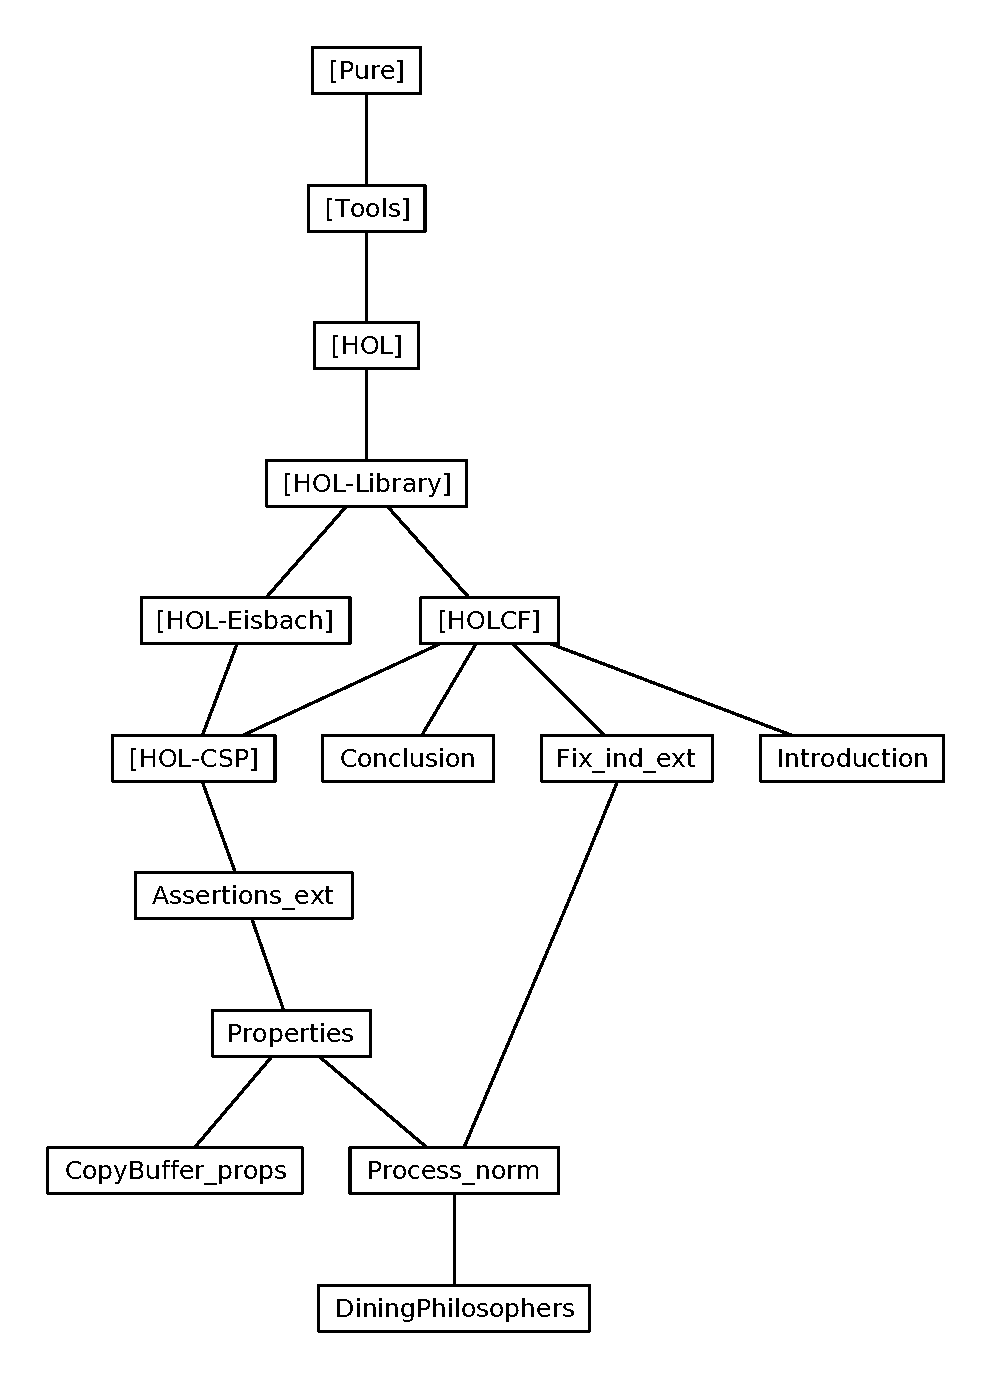
\includegraphics[height=\textheight]{session_graph}
    \caption{The Dependency Graph of the Isabelle Theories.\label{fig:session-graph}}
  \end{figure}
  The rest of this document is automatically generated from the
  formalization in Isabelle/HOL, i.e., all content is checked by
  Isabelle.  Overall, the structure of this document follows the
  theory dependencies (see \autoref{fig:session-graph}): We start with
  the formal framework for verifying stateful security protocols
  (\autoref{cha:verification}). We continue with the setup for
  supporting the high-level protocol specifications language for
  security protocols (the Trac format) and the implementation of the
  fully automated proof tactics (\autoref{cha:trac}). Finally, we
  present examples (\autoref{cha:examples}).

\paragraph{Acknowledgments}
This work was supported by the Sapere-Aude project ``Composec: Secure Composition of Distributed Systems'', grant 4184-00334B of the Danish Council for Independent Research, by the EU H2020 project no. 700321 ``LIGHTest: Lightweight Infrastructure for Global Heterogeneous Trust management in support of an open Ecosystem of Trust schemes'' (lightest.eu) and by the ``CyberSec4Europe'' European Union's Horizon 2020 research and innovation programme under grant agreement No 830929.

\clearpage

\chapter{Stateful Protocol Verification}
\label{cha:verification}
\input{Transactions.tex}
\input{Term_Abstraction.tex}
\input{Stateful_Protocol_Model.tex}
\input{Term_Variants.tex}
\input{Term_Implication.tex}
\input{Stateful_Protocol_Verification.tex}

\chapter{Trac Support and Automation}
\label{cha:trac}
\input{Eisbach_Protocol_Verification.tex}
\input{ml_yacc_lib.tex}
\input{trac_term.tex}
\input{trac_fp_parser.tex}
\input{trac_protocol_parser.tex}
\input{trac.tex}

\chapter{Examples}
\label{cha:examples}
\input{Keyserver.tex}
\input{Keyserver2.tex}
\input{Keyserver_Composition.tex}
\input{PKCS_Model03.tex}
\input{PKCS_Model07.tex}
\input{PKCS_Model09.tex}

% \input{session}


{\small
  \bibliographystyle{abbrvnat}
  \bibliography{root}
}
\end{document}
\endinput 
%%% Local Variables:
%%% mode: latex
%%% TeX-master: t
%%% End:

